%%%%%%%%%%%%%%%%%%%%%%%%
%
% $Autor: Hemanth Jadiswami Prabhakaran $
% $Datum: 2025-06-30 11:18:41Z $
% $Pfad: GitHub/BA25-01-Time-Series/Manual/Chapters/en/03FirstStepsGuide.tex $
% $Version: 1 $
%
% $Project: BA25-Time-Series $
%
%%%%%%%%%%%%%%%%%%%%%%%%



\chapter{First Steps Guide}

\section{Getting Started Overview}

This chapter provides a complete walkthrough for new users to generate their first sales forecast using the Walmart Sales Forecasting System. We will demonstrate the quickest path to results using the cloud-based Prediction Application with the pre-loaded model.

\begin{figure}[H]
	\centering
	\begin{tikzpicture}[node distance=1.5cm and 2.5cm, every node/.style={font=\small}]
	% Title
	\node at (0,6) {\Large\textbf{First Steps Workflow Process}};
	
	% Start
	\node[ellipse, draw, fill=green!20] (start) at (0,4.5) {New User Starts};
	
	% Step 1
	\node[rectangle, draw, fill=blue!20, rounded corners, below=of start] (step1) {Step 1: Access App};
	
	% Step 2
	\node[rectangle, draw, fill=blue!20, rounded corners, below=of step1] (step2) {Step 2: Explore Interface};
	
	% Step 3
	\node[rectangle, draw, fill=blue!20, rounded corners, below=of step2] (step3) {Step 3: Load Model};
	
	% Decision
	\node[diamond, draw, fill=yellow!20, below=of step3] (decision) {Loaded?};
	
	% Troubleshoot (left)
	\node[rectangle, draw, fill=red!20, rounded corners, left=of decision] (trouble) {Troubleshoot};
	
	% Step 4 (right)
	\node[rectangle, draw, fill=blue!20, rounded corners, right=of decision] (step4) {Step 4: Generate Forecast};
	
	% Step 5
	\node[rectangle, draw, fill=blue!20, rounded corners, below=of step4] (step5) {Step 5: Interpret Results};
	
	% Step 6
	\node[rectangle, draw, fill=blue!20, rounded corners, below=of step5] (step6) {Step 6: Download};
	
	% Complete
	\node[rectangle, draw, fill=purple!20, rounded corners, below=of decision] (complete) {Complete!};
	
	% Total Time Box
	\node[rectangle, draw, fill=gray!10, right=of step5, xshift=1.5cm] (total) {Total: 5–10 min};
	
	% Arrows
	\draw[->, thick] (start) -- (step1);
	\draw[->, thick] (step1) -- node[right] {30s} (step2);
	\draw[->, thick] (step2) -- node[right] {2 min} (step3);
	\draw[->, thick] (step3) -- node[right] {10s} (decision);
	
	\draw[->, thick] (decision) -- node[above] {Yes} (step4);
	\draw[->, thick] (step4) -- node[right] {5s} (step5);
	\draw[->, thick] (step5) -- node[right] {2 min} (step6);
	\draw[->, thick] (step6) |- (complete);
	
	\draw[->, thick] (decision) -- node[above] {No} (trouble);
	\draw[->, thick] (trouble) |- (step3);
	
\end{tikzpicture}
	\caption{First Steps Workflow Process}
	\label{fig:firstStepsWorkflow}
\end{figure}

\section{Quick Start: Your First Forecast}

\subsection{Step 1: Access the Prediction Application}

Open your web browser and navigate to the Prediction Application:

\url{https://walmart-sales-prediction-app-py.streamlit.app/}

The application will load within 10-30 seconds, displaying the main interface.

\begin{figure}[H]
	\centering
	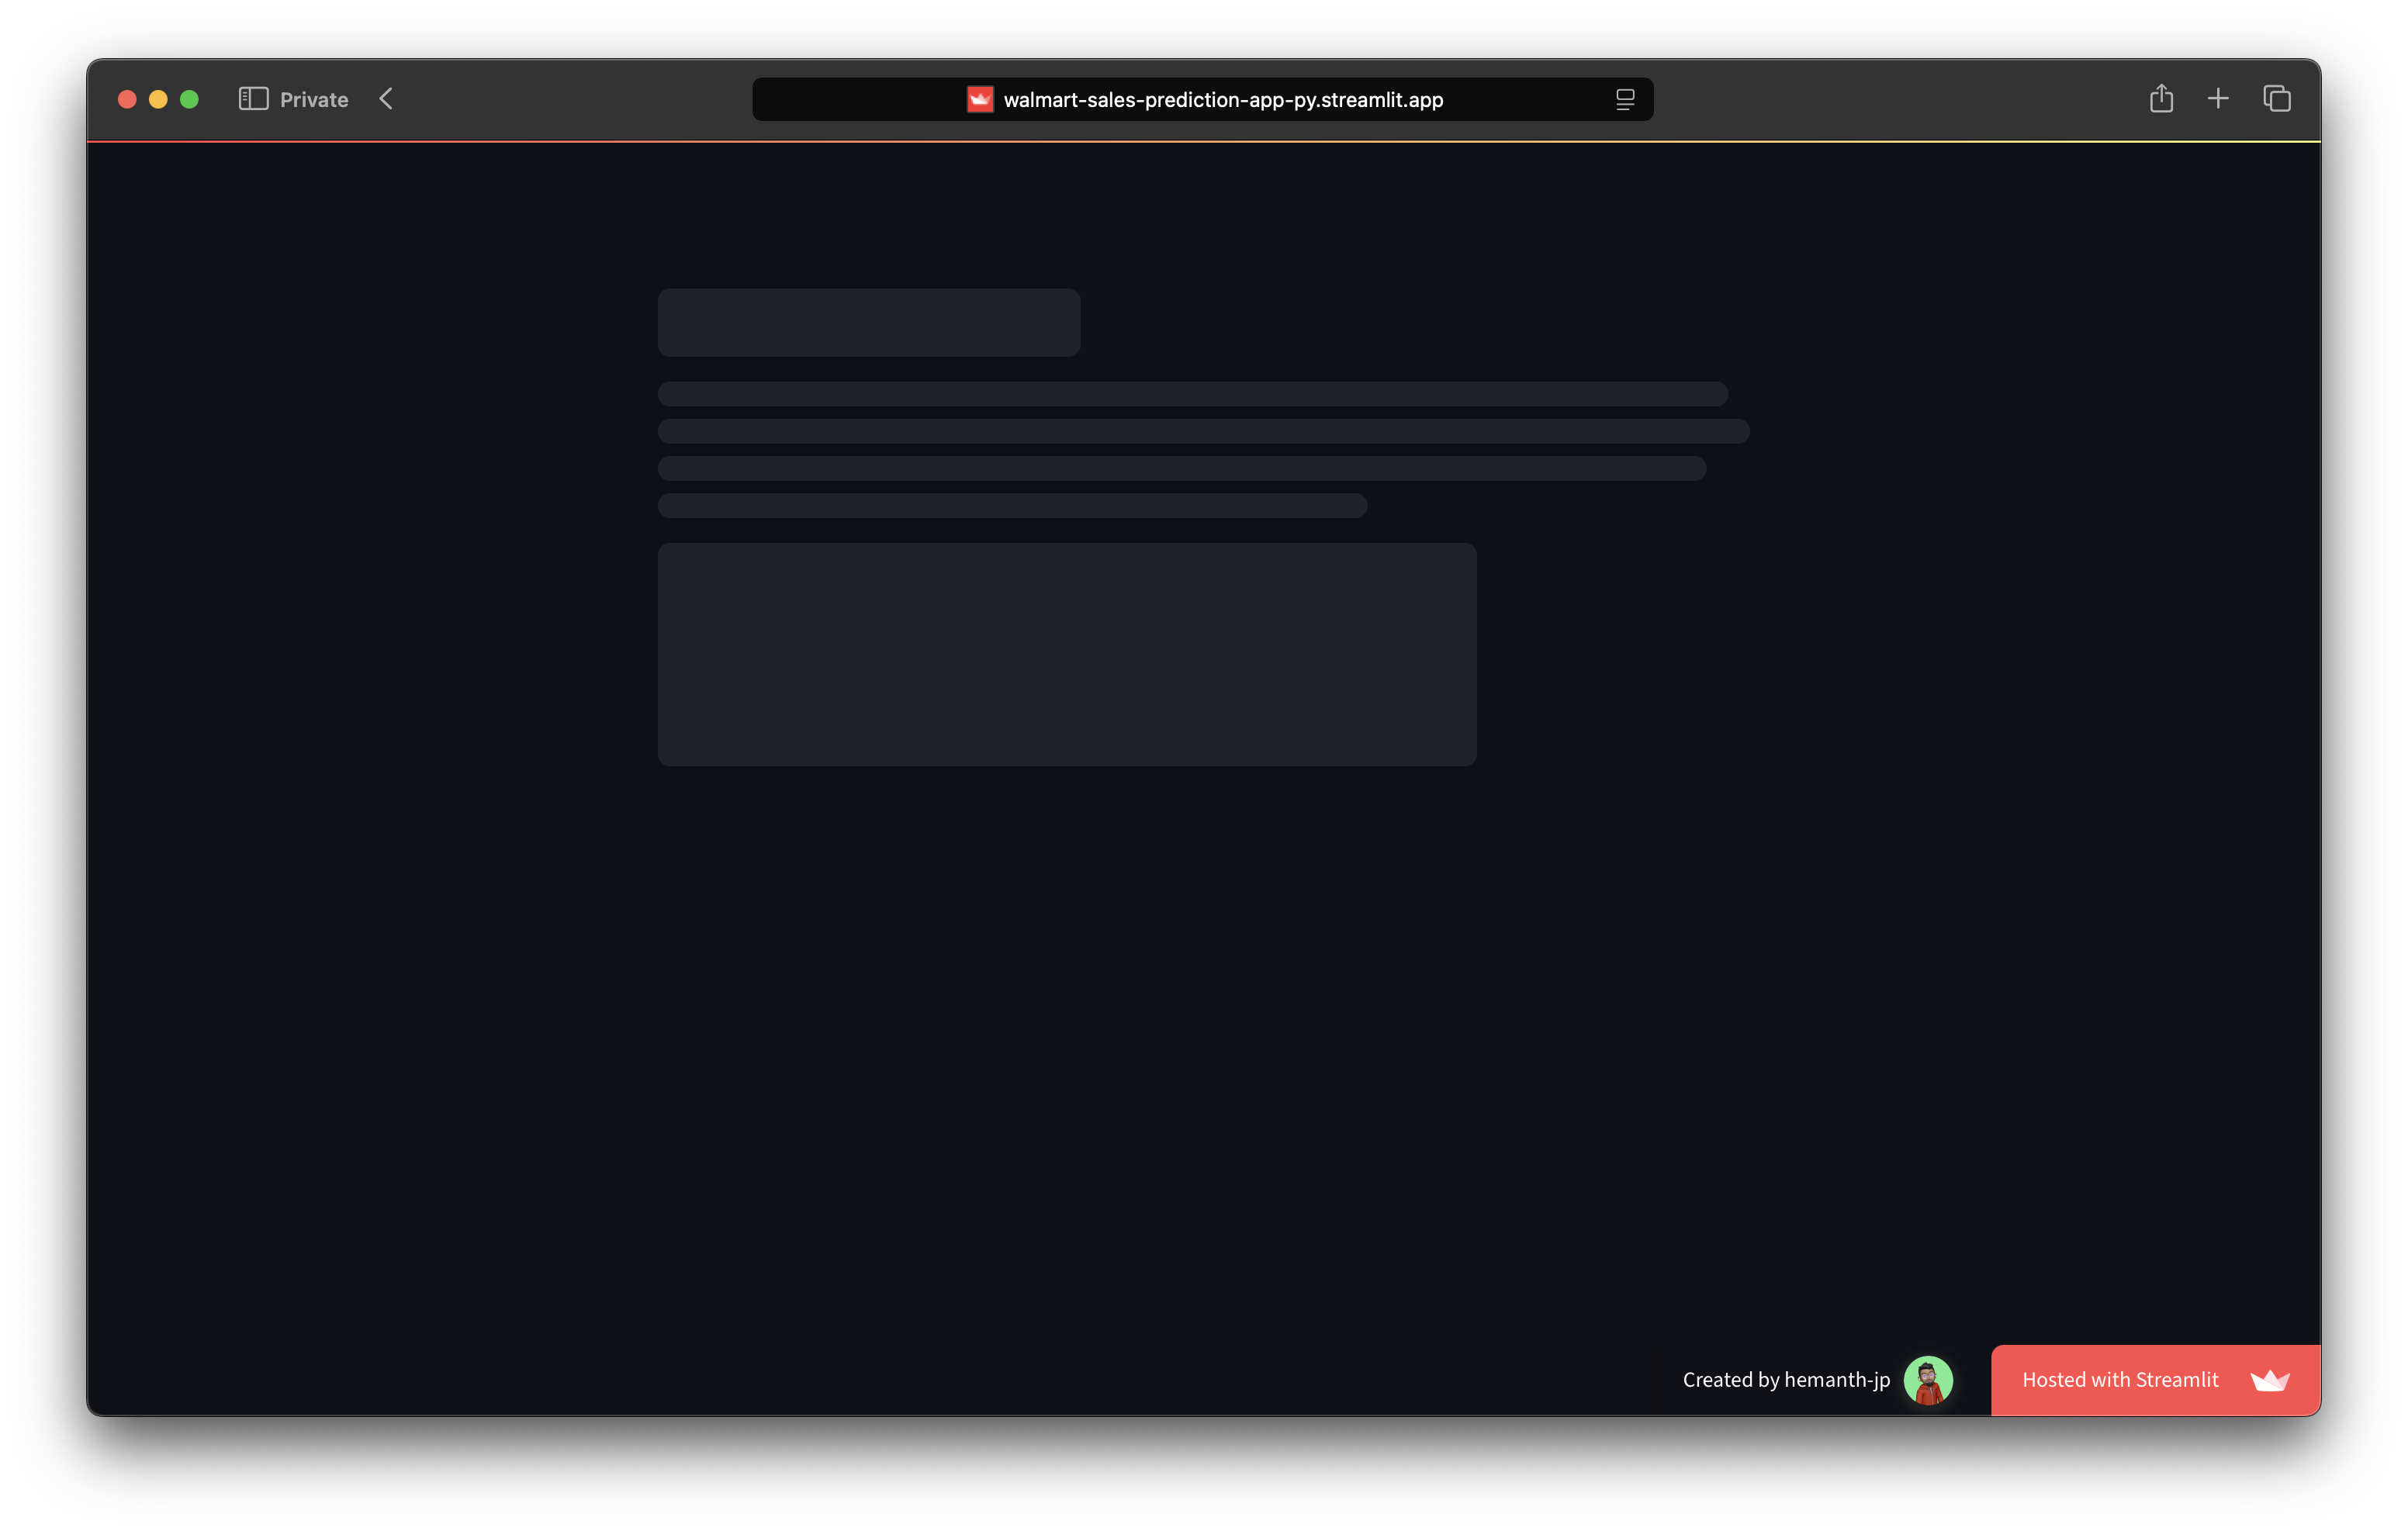
\includegraphics[width=0.9\textwidth]{Images/03FirstStepsGuide/ApplicationLoading.png}
	\caption{Prediction Application Loading Screen}
	\label{fig:applicationLoading}
\end{figure}

\subsection{Step 2: Understand the Interface Layout}

Upon loading, you will see the main interface with these key sections:

\begin{itemize}
	\item \textbf{Header}: Application title and description
	\item \textbf{Model Selection}: Default and custom model options
	\item \textbf{Generate Predictions}: Forecasting controls
	\item \textbf{Results Display}: Charts and data tables (appears after prediction)
\end{itemize}

\begin{figure}[H]
	\centering
	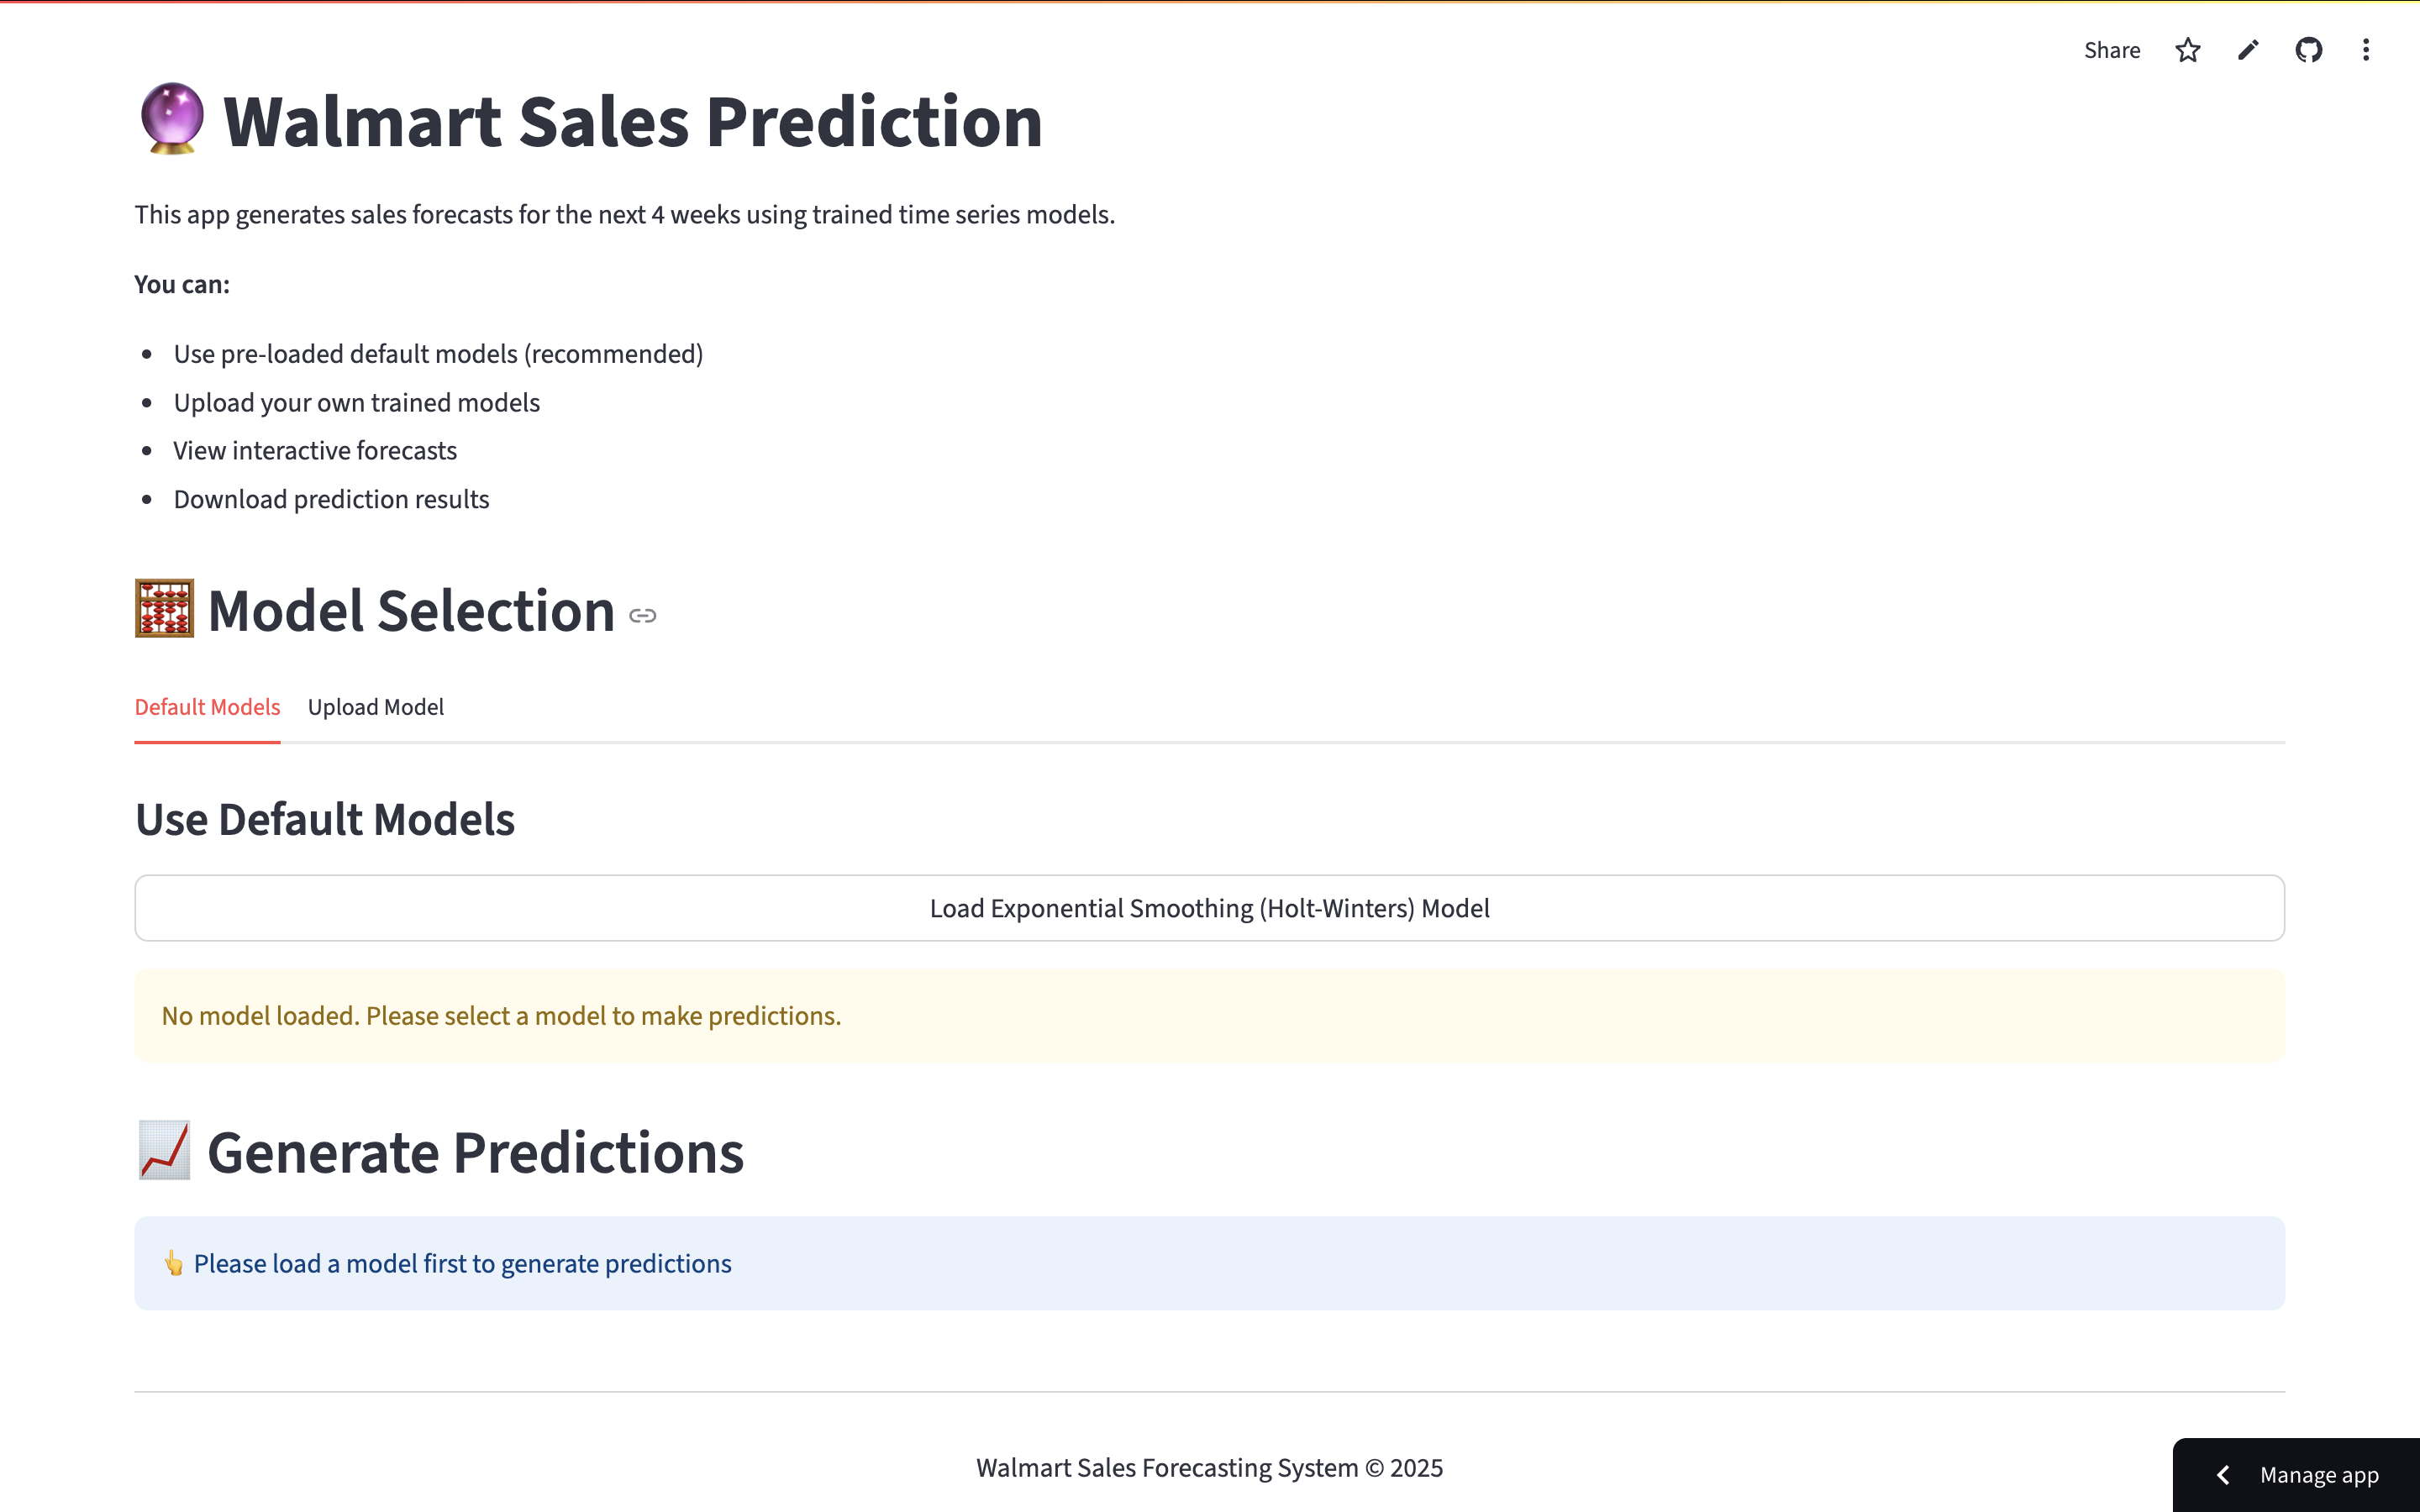
\includegraphics[width=0.9\textwidth]{Images/03FirstStepsGuide/InterfaceLayout.png}
	\caption{Main Interface Layout Overview}
	\label{fig:interface_layout}
\end{figure}

\subsection{Step 3: Load the Default Model}

The system comes with a pre-trained high-performance model. To load it:

\begin{enumerate}
	\item Locate the \textbf{Model Selection} section
	\item Click on the \textbf{Default Models} tab
	\item Click the \textbf{Load Exponential Smoothing (Holt-Winters) Model} button
	\item Wait for the success message: "  Exponential Smoothing (Holt-Winters) model loaded successfully!"
\end{enumerate}

\begin{figure}[H]
	\centering
	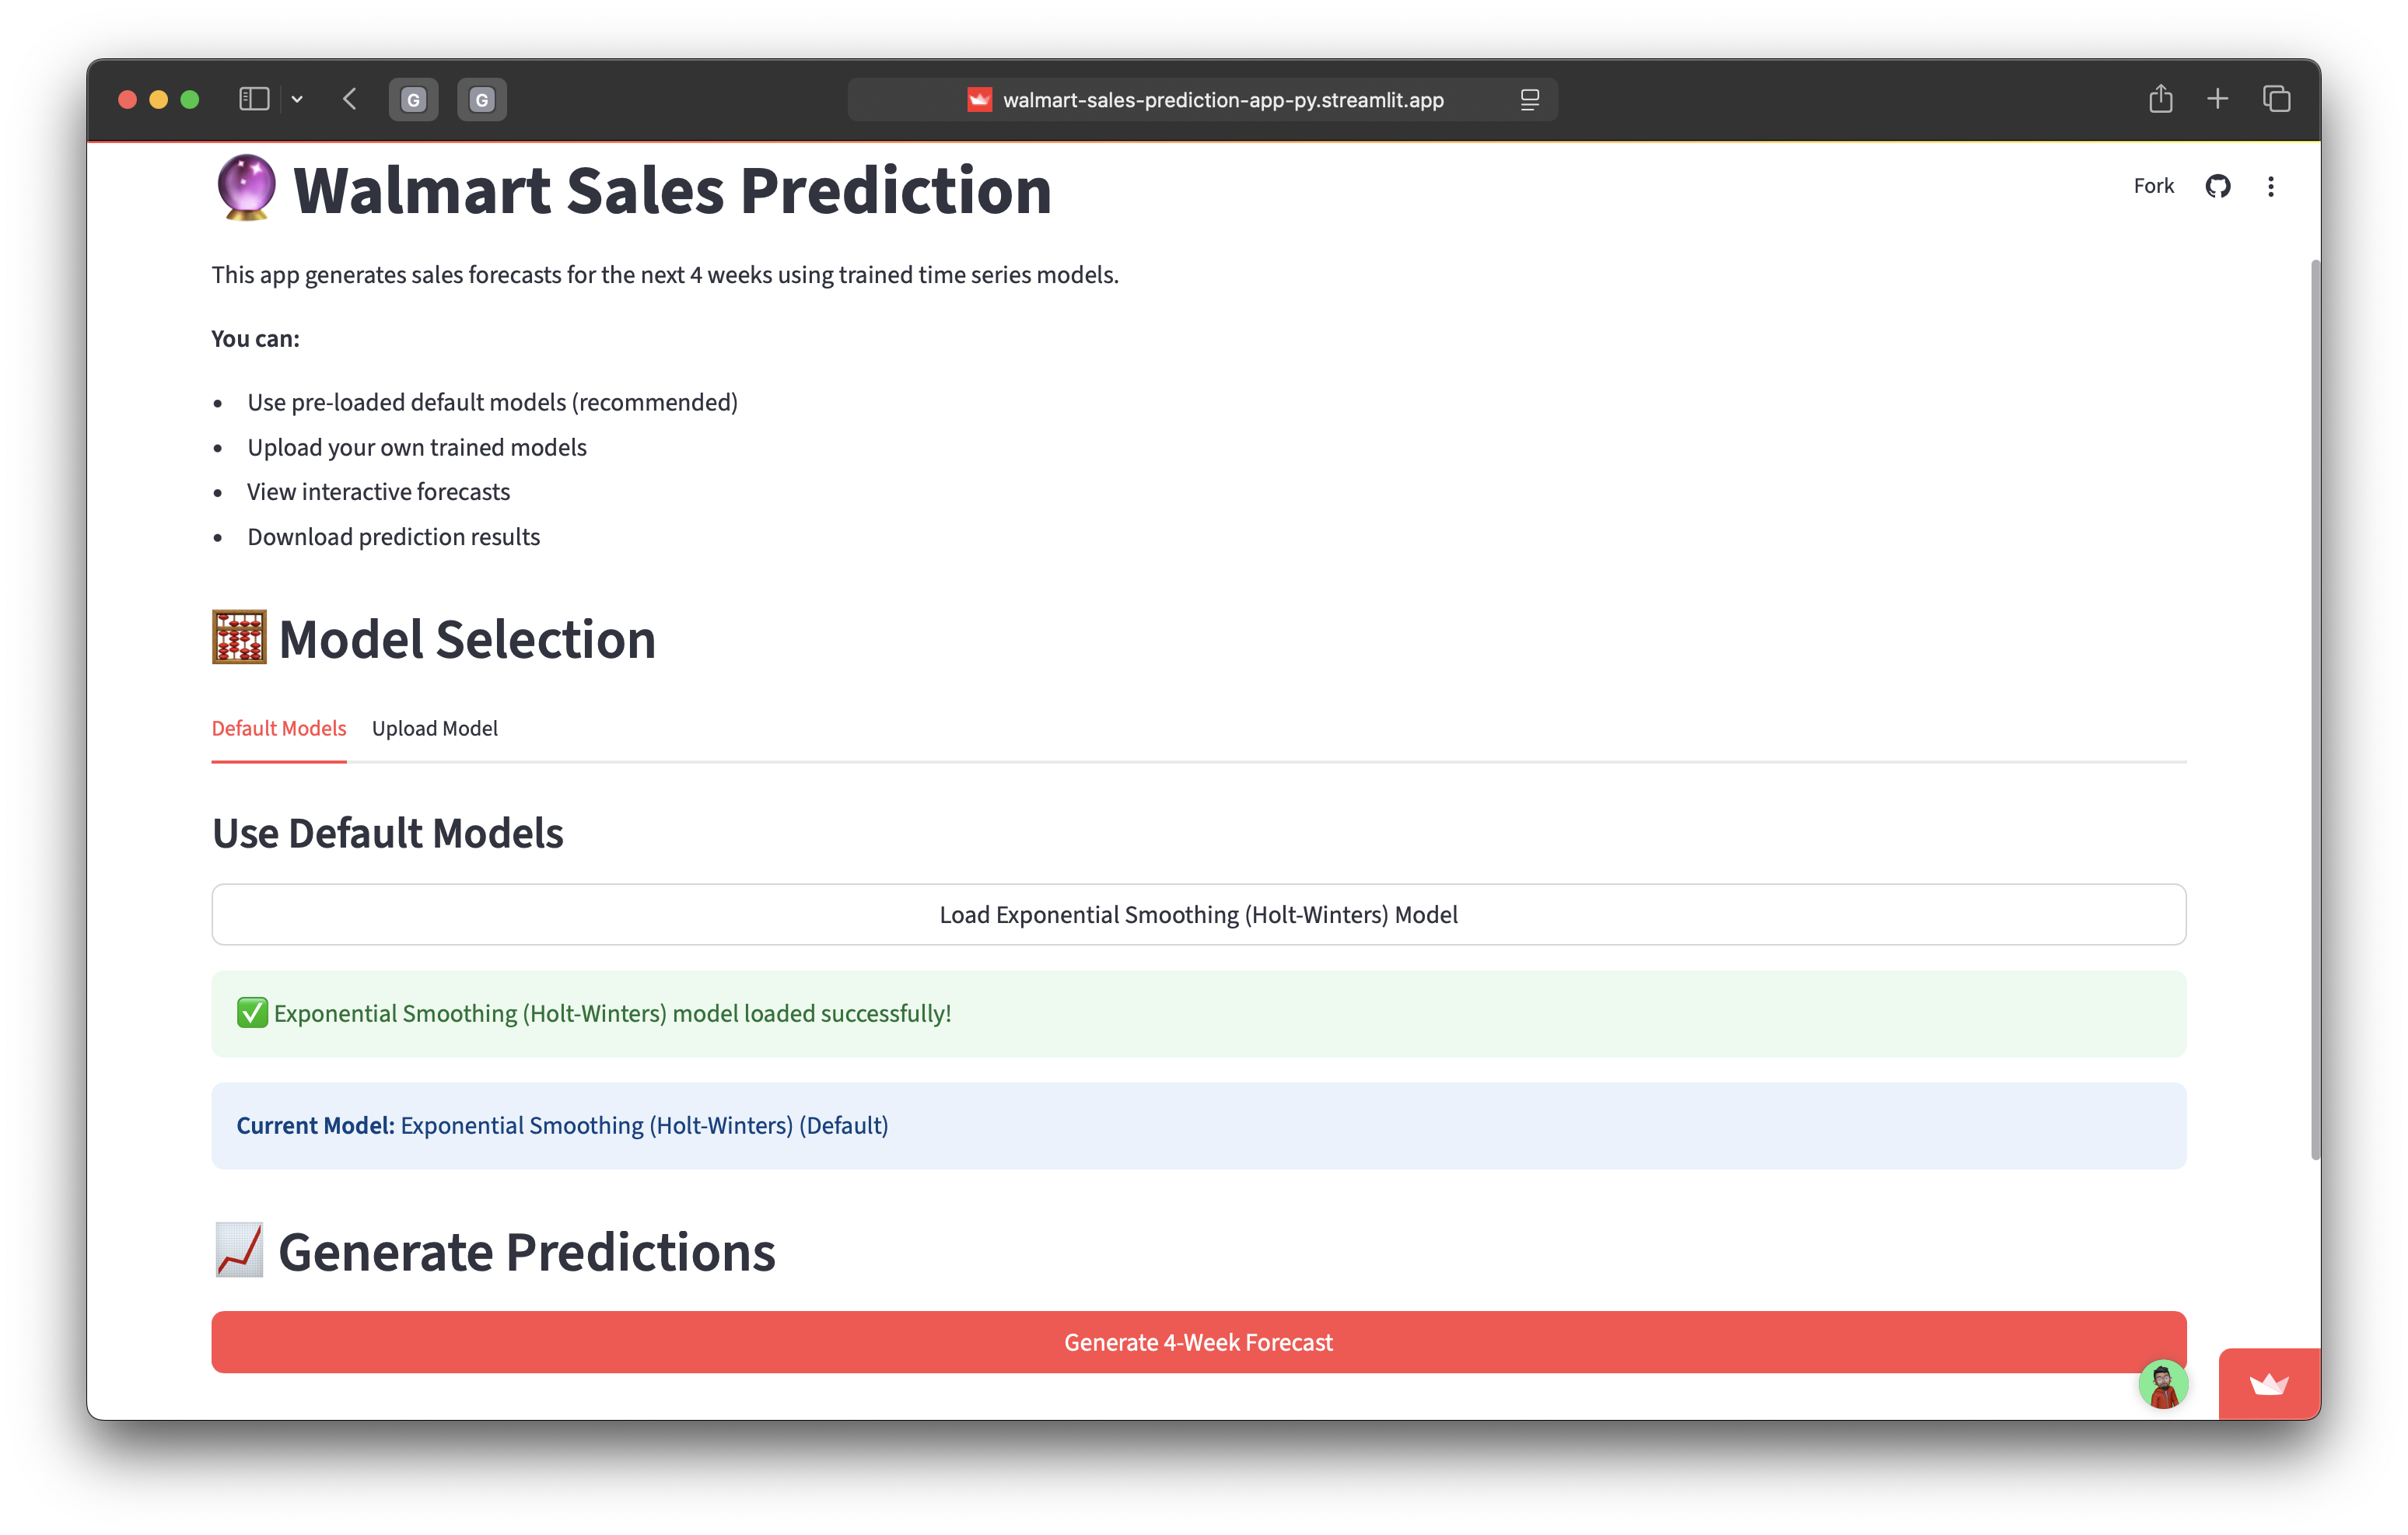
\includegraphics[width=0.9\textwidth]{Images/03FirstStepsGuide/ModelLoading.png}
	\caption{Default Model Loading Process}
	\label{fig:model_loading}
\end{figure}

\subsection{Step 4: Generate Your First Forecast}

With the model loaded, generate predictions:

\begin{enumerate}
	\item Scroll down to the \textbf{Generate Predictions} section
	\item Click the \textbf{Generate 4-Week Forecast} button
	\item The system will process for a few seconds
	\item Results will appear below with charts and data tables
\end{enumerate}

\begin{figure}[H]
	\centering
	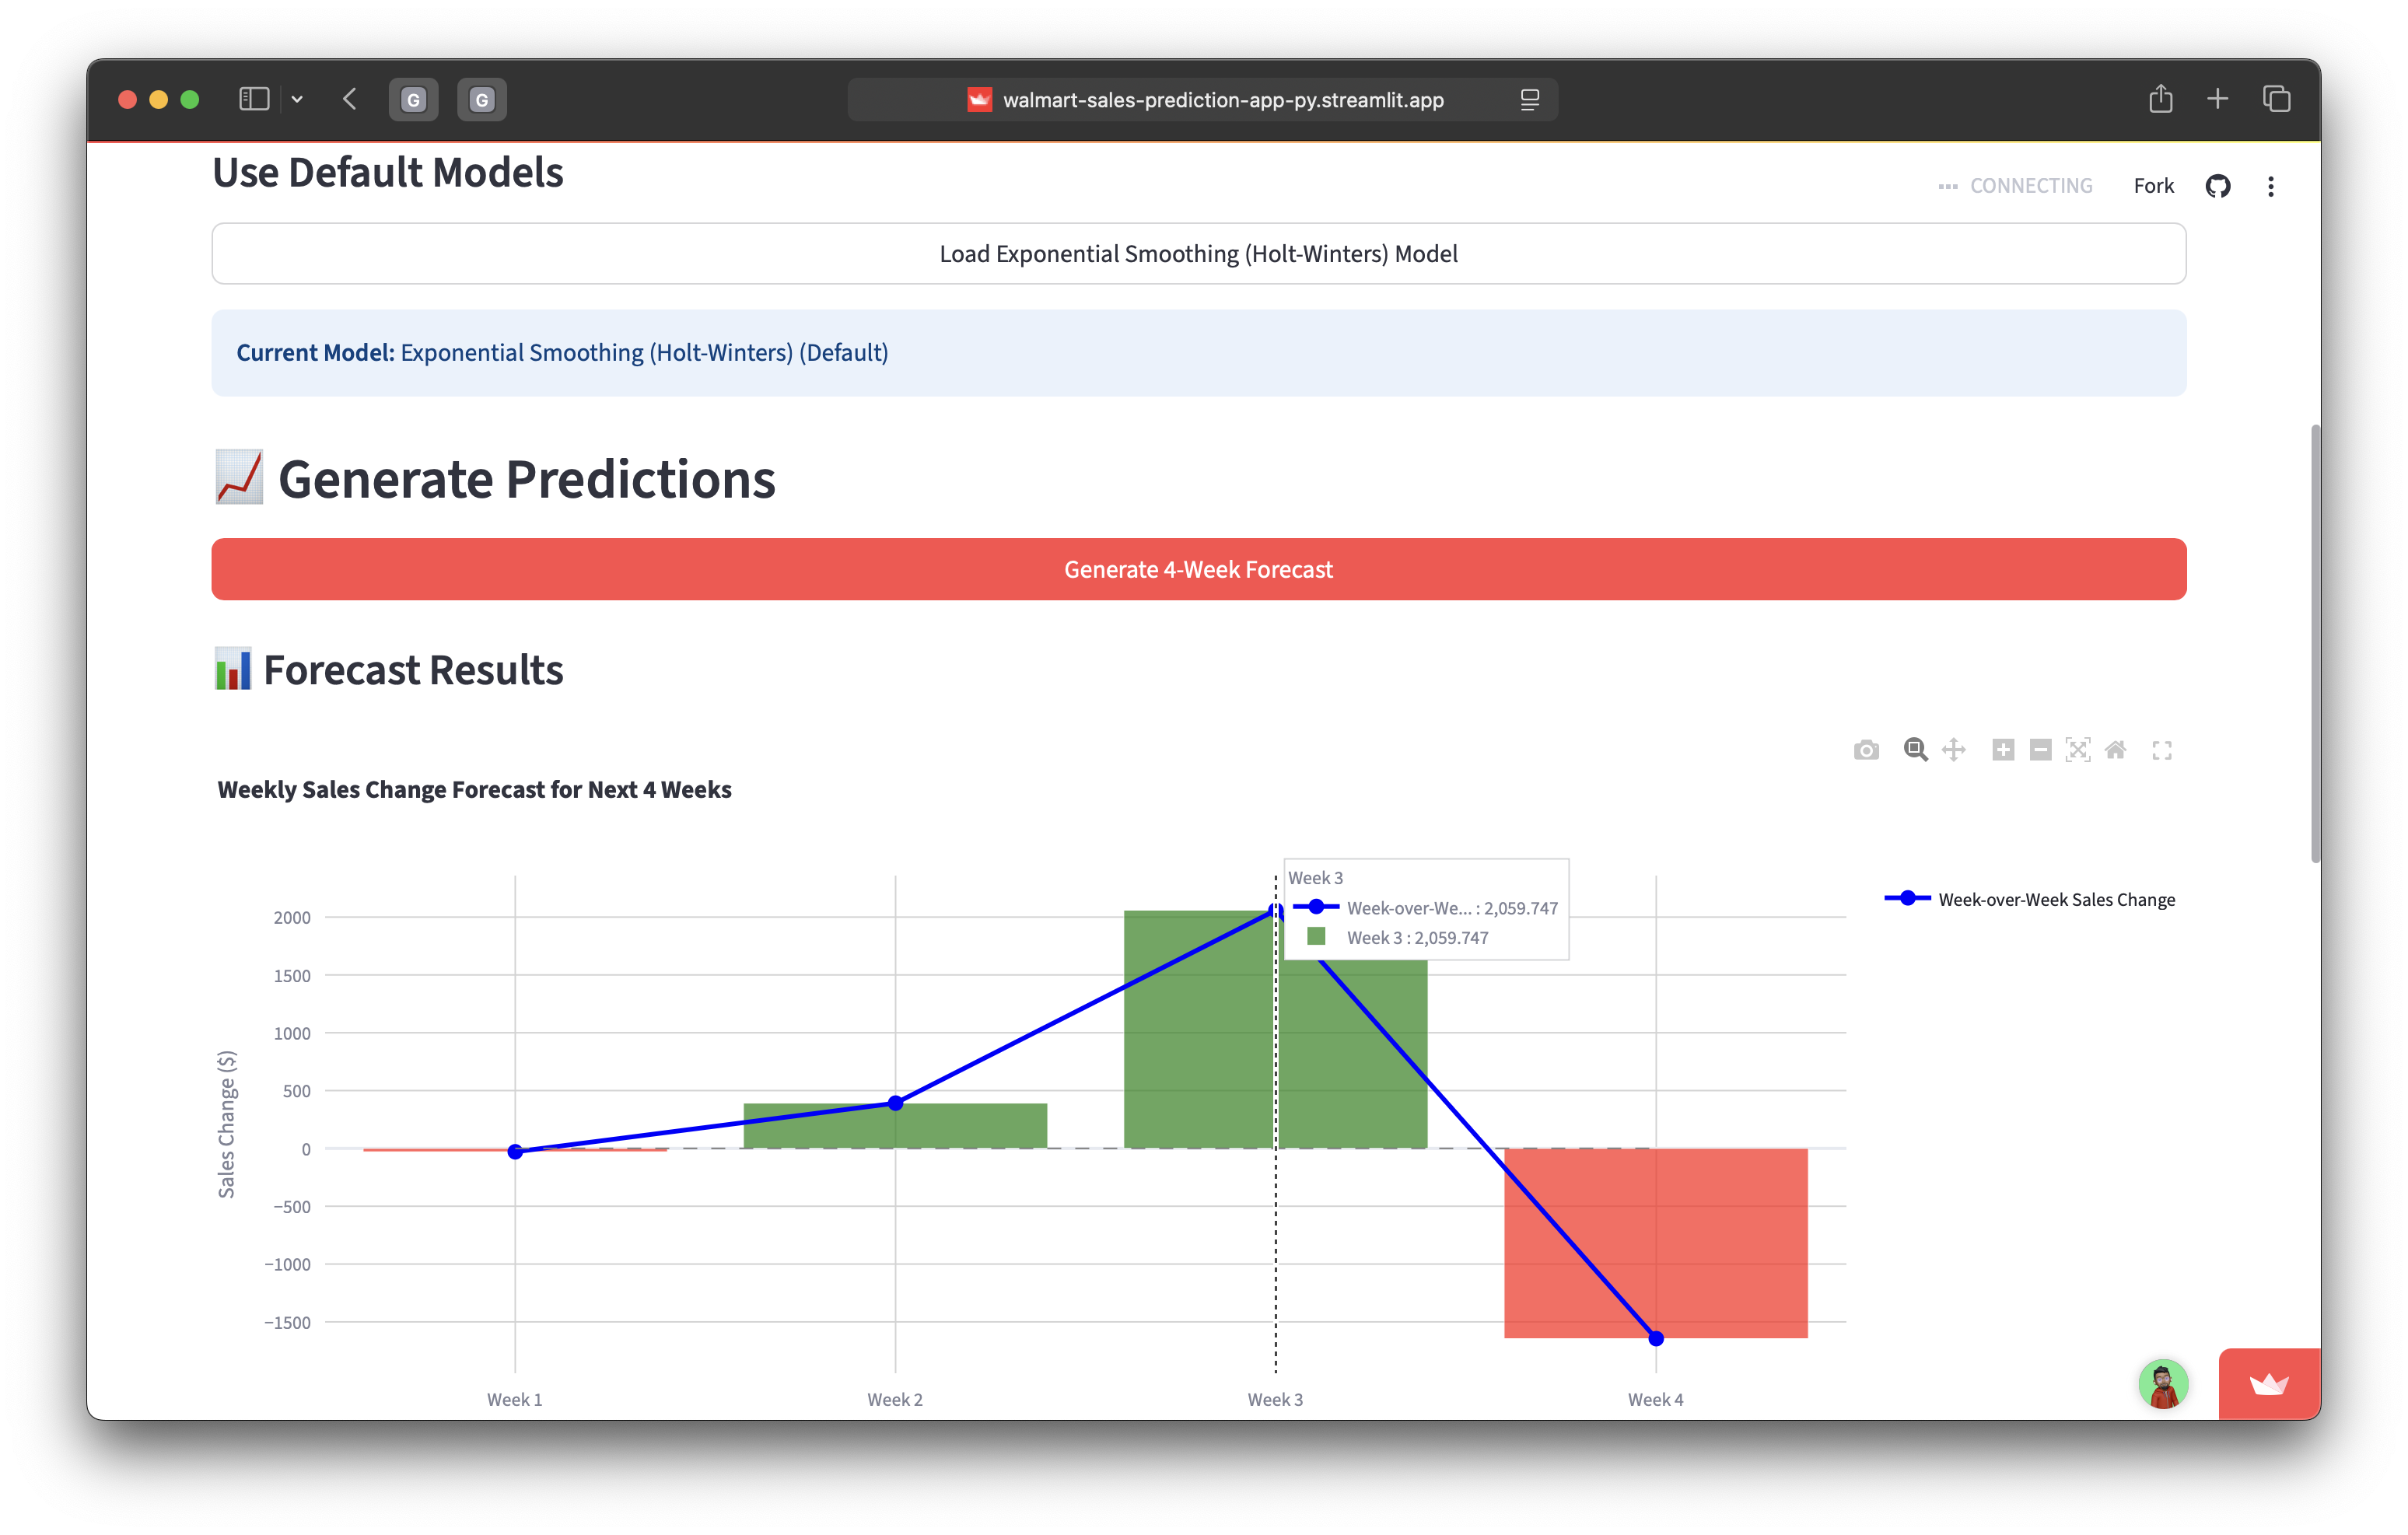
\includegraphics[width=0.9\textwidth]{Images/03FirstStepsGuide/GeneratingForecast.png}
	\caption{Forecast Generation Process}
	\label{fig:generating_forecast}
\end{figure}

\section{Understanding Your First Results}

\subsection{Forecast Interpretation}

The generated forecast shows \textbf{week-over-week sales changes}, not absolute sales values:

\begin{itemize}
	\item \textbf{Positive Values} (Green): Sales increase from previous week
	\item \textbf{Negative Values} (Red): Sales decrease from previous week
	\item \textbf{Dollar Amounts}: Change in sales dollars, not total sales
\end{itemize}

\begin{figure}[H]
	\centering
	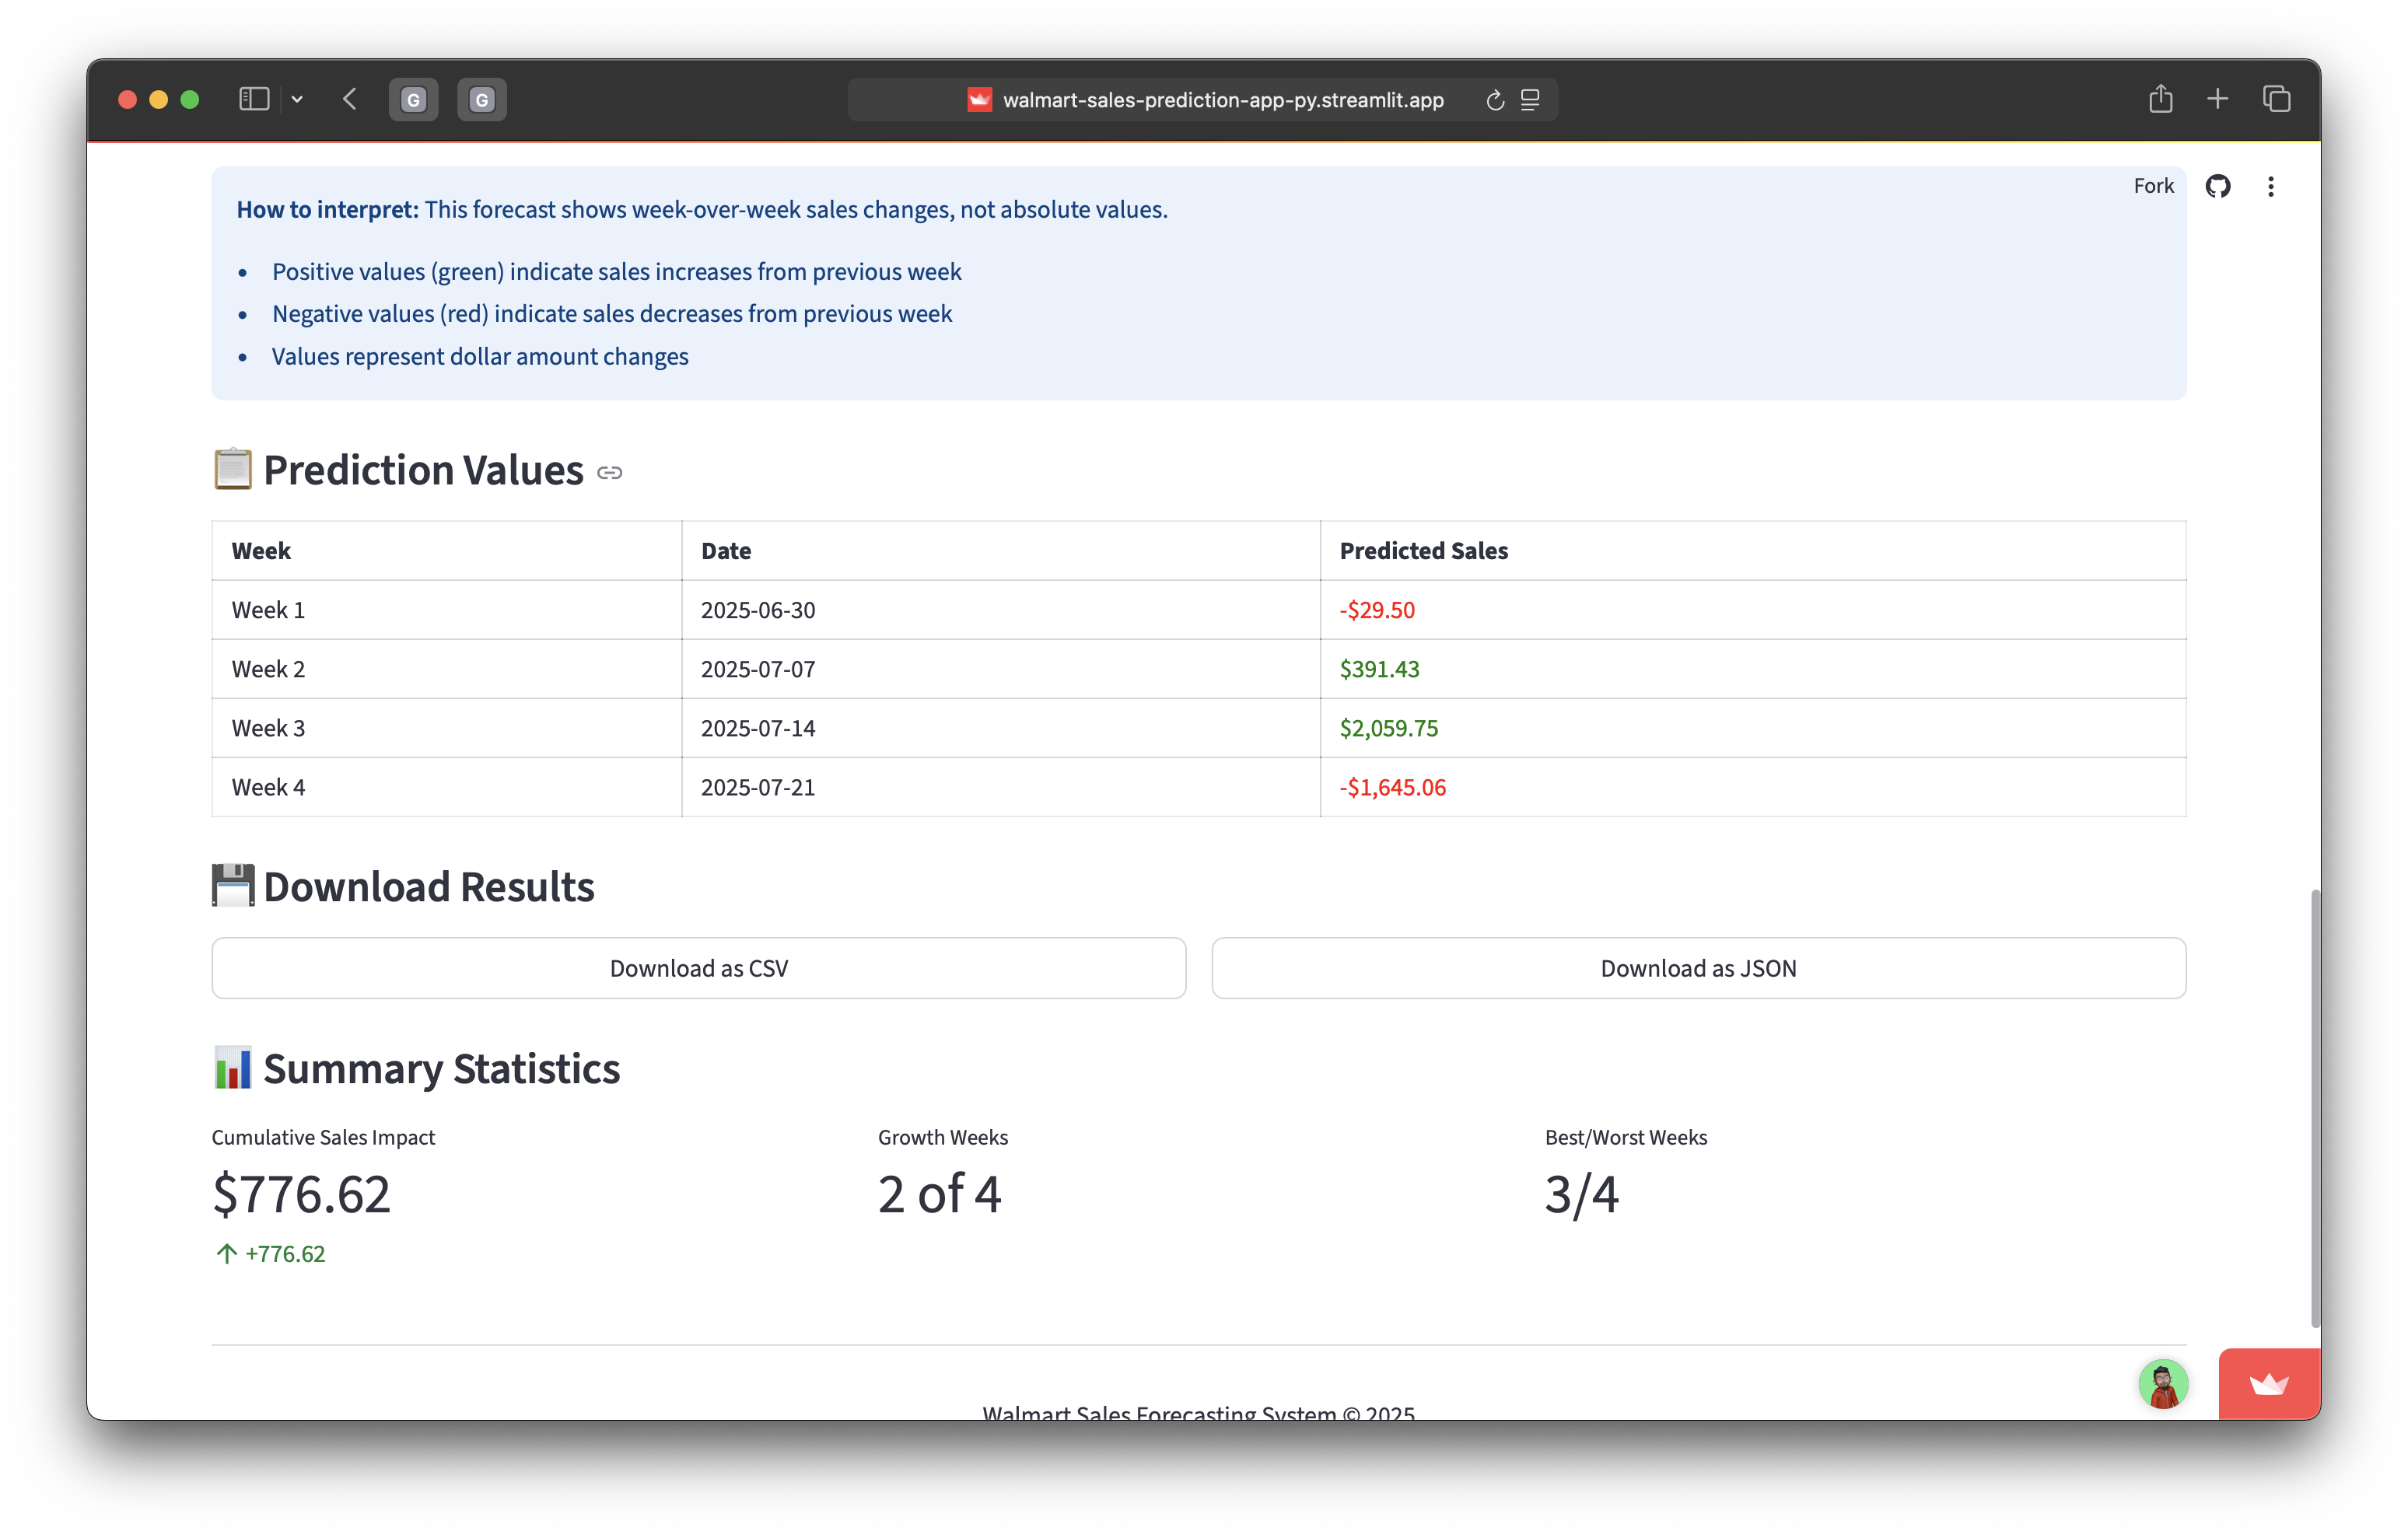
\includegraphics[width=0.9\textwidth]{Images/03FirstStepsGuide/ForecastResults.png}
	\caption{Sample Forecast Results with Interpretation}
	\label{fig:forecast_results}
\end{figure}

\subsection{Interactive Visualization}

The forecast chart provides interactive features:

\begin{itemize}
	\item \textbf{Hover Information}: Point your mouse over data points for detailed values
	\item \textbf{Zoom}: Use mouse wheel or touch gestures to zoom in/out
	\item \textbf{Pan}: Click and drag to move around the chart
	\item \textbf{Color Coding}: Green bars for growth, red bars for decline
\end{itemize}

\subsection{Data Table Review}

Below the chart, examine the detailed data table:

\begin{table}[H]
	\centering
	\begin{tabular}{|c|c|c|}
		\hline
		\textbf{Week} & \textbf{Date} & \textbf{Predicted Sales} \\
		\hline
		Week 1 & 2025-06-29 & \$1,234.56 \\
		Week 2 & 2025-07-06 & -\$567.89 \\
		Week 3 & 2025-07-13 & \$890.12 \\
		Week 4 & 2025-07-20 & \$345.67 \\
		\hline
	\end{tabular}
	\caption{Example Forecast Data Table}
	\label{tab:forecast_example}
\end{table}

\section{Exploring Summary Statistics}

\subsection{Performance Metrics}

Review the model performance information displayed:

\begin{itemize}
	\item \textbf{Cumulative Sales Impact}: Total predicted change across all weeks
	\item \textbf{Growth Weeks}: Number of weeks with positive sales changes
	\item \textbf{Best/Worst Weeks}: Which weeks show strongest/weakest performance
\end{itemize}

\begin{figure}[H]
	\centering
	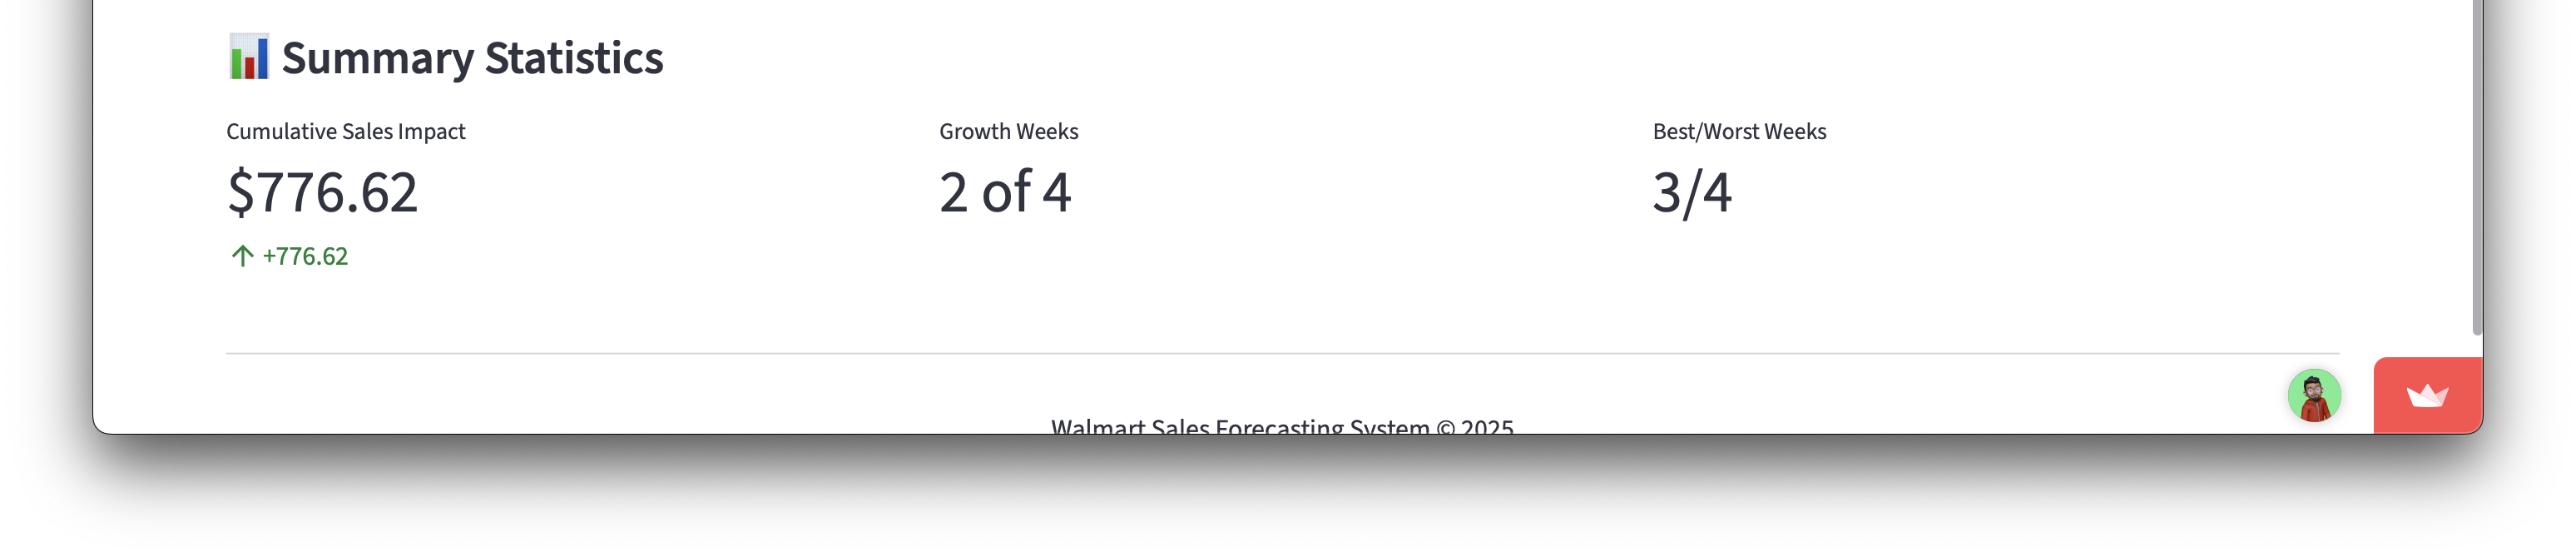
\includegraphics[width=0.9\textwidth]{Images/03FirstStepsGuide/SummaryStatistics.png}
	\caption{Summary Statistics Display}
	\label{fig:summary_statistics}
\end{figure}

\subsection{Model Quality Indicator}

The default model shows excellent performance:

\begin{itemize}
	\item \textbf{Normalized WMAE}: 3.58\% (Excellent - less than 5\% error)
	\item \textbf{Quality Rating}: High confidence for business forecasting decisions
\end{itemize}

\section{Downloading Your Results}

\subsection{Export Options}

Save your forecast results for further analysis:

\begin{enumerate}
	\item Scroll to the \textbf{Download Results} section
	\item Choose your preferred format:
	\begin{itemize}
		\item \textbf{CSV Format}: For Excel or data analysis tools
		\item \textbf{JSON Format}: For programming or API integration
	\end{itemize}
	\item Click the corresponding download button
	\item Save the file to your desired location
\end{enumerate}

\begin{figure}[H]
	\centering
	
\includegraphics[width=0.9\textwidth]{Images/03FirstStepsGuide/DownloadOptions.png}
	\caption{Forecast Results Download Options}
	\label{fig:download_options}
\end{figure}

\section{Next Steps After Your First Forecast}

\subsection{Immediate Actions}

After completing your first forecast:

\begin{enumerate}
	\item \textbf{Analyze Results}: Review the forecast values and trends
	\item \textbf{Save Data}: Download results in your preferred format
	\item \textbf{Share Insights}: Export charts for presentations or reports
\end{enumerate}

\subsection{Advanced Exploration}

Once comfortable with basic forecasting:

\begin{itemize}
	\item \textbf{Try Different Models}: If you have your own model .pkl (Auto Arima / Exponential Smoothing) explore custom models
	\item \textbf{Train Custom Models}: Use the Training Application for specific datasets
	\item \textbf{Upload Your Models}: Use personally trained models for prediction
\end{itemize}

\section{Common First-Time Questions}

\subsection{Understanding Predictions}

\textbf{Q: Why are some values negative?}\\
\textbf{A:} Negative values indicate sales decreases from the previous week, which is normal in retail patterns.

\textbf{Q: How accurate are these predictions?}\\
\textbf{A:} The default model has a 3.58\% normalized WMAE, indicating excellent accuracy for business forecasting.

\textbf{Q: Can I predict further than 4 weeks?}\\
\textbf{A:} The current system is optimized for 4-week forecasts. Longer periods may require model retraining and code update.

\subsection{Technical Questions}

\textbf{Q: Do I need to install anything?}\\
\textbf{A:} No, the cloud version requires only a web browser. Local installation is optional for advanced users.

\textbf{Q: Can I use my own data?}\\
\textbf{A:} Yes, use the Training Application to train models with your dataset, then upload them to the Prediction Application.

\textbf{Q: What if the application stops working?}\\
\textbf{A:} Refresh the browser page. Cloud applications may timeout after extended idle periods.

\section{Troubleshooting First Steps}

\subsection{Application Loading Issues}

\textbf{Problem}: Application takes too long to load or shows errors.\\
\textbf{Solution}:
\begin{itemize}
	\item Check internet connection stability
	\item Try refreshing the browser page
	\item Clear browser cache if problems persist
	\item Use a different browser (Chrome recommended)
\end{itemize}

\subsection{Model Loading Failures}

\textbf{Problem}: Default model fails to load with error messages.\\
\textbf{Solution}:
\begin{itemize}
	\item Refresh the application completely
	\item Try again after a few minutes (server may be busy)
	\item Check if you're using a supported browser
\end{itemize}

\subsection{Prediction Generation Errors}

\textbf{Problem}: Forecast generation fails or returns errors.\\
\textbf{Solution}:
\begin{itemize}
	\item Ensure the model is properly loaded (green success message)
	\item Refresh the application and retry
	\item Check that you clicked the correct forecast button
\end{itemize}

\section{Building Confidence with Practice}

\subsection{Recommended Practice Steps}

To build familiarity with the system:

\begin{enumerate}
	\item \textbf{Generate Multiple Forecasts}: Run several predictions to see consistent results
	\item \textbf{Explore Interface Features}: Click through different tabs and options
	\item \textbf{Download Results}: Practice exporting data in different formats
	\item \textbf{Review Documentation}: Read detailed interface descriptions in Chapter 4
\end{enumerate}

\subsection{Learning Path}

Progress through these stages:

\begin{itemize}
	\item \textbf{Beginner}: Use default model for basic forecasting
	\item \textbf{Intermediate}: Explore custom model uploads and different formats
	\item \textbf{Advanced}: Train your own models using the Training Application
\end{itemize}

\section{Summary}

This first steps guide demonstrated:

\begin{itemize}
	\item How to access the cloud-based Prediction Application
	\item Loading and using the default high-performance model
	\item Generating your first 4-week sales forecast
	\item Interpreting week-over-week sales change predictions
	\item Downloading results for further analysis
	\item Common troubleshooting for first-time users
\end{itemize}

You are now ready to explore the advanced features covered in subsequent chapters or begin using the system for regular forecasting activities.

